This module had to realise control of robot wheels. Since designed robot uses
Dual 12Volt 2.8Amp H Bridge Motor Drive MD25 \footnote{\url{http://www.robot-electronics.co.uk/htm/md25i2c.htm}}, controlling the board was realised using I2C bus system mode.
Generally this module had to realize following actions:
\begin{itemize}
	\item drive motors by setting individual speeds for both wheels;
	\item get heading of the robot by reading encoder values.
\end{itemize}
These requirements led to splitting the whole module into two blocks:  one being responsible for driving motors and another for reading/writing encoders.

\begin{figure}[!ht]
	\centering
	\begin{tikzpicture}[node distance = 2cm, auto]
	\tikzstyle{block} = [rectangle, draw, fill=blue!20, 
	text width=5em, text centered, rounded corners, minimum height=4em]
	\tikzstyle{line} = [draw, -latex']
	% Place nodes
	\node [block] (navigator) {Motion navigator};
	\node [block, below of=navigator, xshift=-1.5cm] (motors) {Motors};
	\node [block, below of=navigator, xshift= 1.5cm] (encoders) {Encoders};
	% Draw edges
	\path [line] (navigator) -| (motors);
	\path [line] (navigator) -| (encoders);
	\end{tikzpicture}
	\caption{Motion module structure}
	\label{fig:motion_structure}
\end{figure}

\paragraph{Controlling motors}

All communications between high level functions and motors were realized via  I2C bus command register.
The MD25 has 17 registers numbered 0 to 16 as follows:
\begin{table}[!h]
	\begin{tabular}{@{}llll@{}}
		\toprule
		\textbf{Register} & \textbf{Name}     & \textbf{Read/Write} & \textbf{Description}                                             \\ \midrule
		0                 & Speed1            & R/W                 & Motor1 speed (mode 0,1) or speed (mode 2,3)                      \\
		1                 & Speed2/Turn       & R/W                 & Motor2 speed (mode 0,1) or turn (mode 2,3)                       \\
		2                 & Enc1a             & Read only           & Encoder 1 position, 1st byte (highest),   \\
		3                 & Enc1b             & Read only           & Encoder 1 position, 2nd byte                                     \\
		4                 & Enc1c             & Read only           & Encoder 1 position, 3rd byte                                     \\
		5                 & Enc1d             & Read only           & Encoder 1 position, 4th (lowest byte)                            \\
		6                 & Enc2a             & Read only           & Encoder 2 position, 1st  byte (highest),  \\
		7                 & Enc2b             & Read only           & Encoder 2 position, 2nd byte                                     \\
		8                 & Enc2c             & Read only           & Encoder 2 position, 3rd byte                                     \\
		9                 & Enc2d             & Read only           & Encoder 2 position, 4th byte (lowest byte)                       \\
		10                & Battery volts     & Read only           & The supply battery voltage                                       \\
		11                & Motor 1 current   & Read only           & The current through motor 1                                      \\
		12                & Motor 2 current   & Read only           & The current through motor 2                                      \\
		13                & Software Revision & Read only           & Software Revision Number                                         \\
		14                & Acceleration rate & R/W                 & Optional Acceleration register                                   \\
		15                & Mode              & R/W                 & Mode of operation (see below)                                    \\
		16                & Command           & Write only          & Used for reset of encoder counts and module address changes      \\ \bottomrule
	\end{tabular}
	\caption{The MD25 register values and description}
\end{table}

\newpage
For controlling the motors, registers 0, 1 and 15 are used. Firstly, when initializing motor control, mode register (15) is modified.
The mode register selects which mode of operation and I2C data input type the user requires. Here the type 3 was chosen and writing this value 
to the mode register makes enables turn mode: "speed1" controls both motors \textit{speed}, and "speed2" becomes the \textit{turn} value. 
Data is in the range of -128 for full reverse, 0 for stop and 127 for full forward speed of motors.

It is worth to mention, that turn mode looks at the speed register to decide if the direction is forward or reverse. Then it applies a subtraction or addition of the turn value on either motor. If the direction is forward:
\begin{table}[!ht]
	\centering
	\begin{tabular}{lcl}
		motor speed1 & = & speed - turn,\\
		motor speed2 & = & speed + turn,
	\end{tabular}
\end{table}

else the direction is reverse:
\begin{table}[!ht]
	\centering
	\begin{tabular}{lcl}
		motor speed1 & = & speed + turn,\\
		motor speed2 & = & speed - turn.
	\end{tabular}
\end{table}

Manipulating mentioned registers, 4 main motor controlling functions were implemented as seen in figure \ref{fig:motor_structure}.
\begin{figure}[!ht]
	\centering
	\begin{tikzpicture}[node distance = 2cm, auto]
	\tikzstyle{block} = [rectangle, draw, fill=blue!20, 
	text width=5em, text centered, rounded corners, minimum height=4em]
	\tikzstyle{line} = [draw, -latex']
	% Place nodes
	\node [block] (motors) {Motors};
	\node [block, below of=navigator, xshift=-1.5cm] (stop) {Stop Motors};
	\node [block, left of=stop, node distance = 3 cm] (drive) {Drive Motors};
	\node [block, below of=navigator, xshift=1.5cm] (left) {Turn left};
	\node [block, right of=left,  node distance = 3 cm] (right) {Turn right};
	% Draw edges
	\path [line] (motors) -| (drive);
	\path [line] (motors) -| (stop);
	\path [line] (motors) -| (left);
	\path [line] (motors) -| (right);
	\end{tikzpicture}
	\caption{Motor controlling functions}
	\label{fig:motor_structure}
\end{figure}

\paragraph{Controlling encoders}

For controlling the encoders, registers 2-9 and 16 are used.
Manipulating mentioned registers, 3 main encoder controlling functions were implemented, which are presented figure \ref{fig:encoder_structure}.
\begin{figure}[!ht]
	\centering
	\begin{tikzpicture}[node distance = 2cm, auto]
	\tikzstyle{block} = [rectangle, draw, fill=blue!20, 
	text width=5em, text centered, rounded corners, minimum height=4em]
	\tikzstyle{line} = [draw, -latex']
	% Place nodes
	\node [block] (encoders) {Encoders};
	\node [block, below of=navigator, xshift=-1.5cm] 	(rleft) {Read right encoder};
	\node [block, left of=stop, node distance = 3 cm] 	(lleft) {Read left encoder};
	\node [block, below of=navigator, xshift=1.5cm] 	(reset) {Reset both encoders};
	\node [block, right of=left,  node distance = 3 cm] (angle) {Get robot heading};
	% Draw edges
	\path [line] (encoders) -| (rleft);
	\path [line] (encoders) -| (lleft);
	\path [line] (encoders) -| (reset);
	\path [line] (encoders) -| (angle);
	\end{tikzpicture}
	\caption{Motor controlling functions}
	\label{fig:encoder_structure}
\end{figure}


\paragraph{Heading calculation}

Robot heading calculation is implemented realising two formulas stated below.
%$$
%radiansPerCount = \pi* (wheelDiameter/trackWidth) / countsPerRevolution
%$$
%and
%$$
%heading = (countsEncoderRight - countsEncoderLeft) * radiansPerCount
%$$ 

\begin{eqnarray}
rad_{pc}  = & \pi \cdot \frac{ d_{wheel} }{ d_{track} } / c_{pr}	,			\\
\theta_{h} = & (ce_{r} - ce_{l} ) \cdot rad_{pc} ,
\label{eq:rb_heading}
\end{eqnarray}
where 
\begin{itemize}
	\item $rad_{pc}$ - radians per one encoder count,
	\item $d_{wheel}$ - wheel diameter,
	\item $d_{track}$ - track width (or distance between the wheels), %as in figure \ref{fig:rb_wheel_graph},
	\item $c_{pr}$ - encoder counts per output shaft (wheel) turn,
	\item $ce_{r}$ - right encoder counts,
	\item $ce_{l}$ - left encoder counts,
	\item $\theta_{rh}$ - robot heading in radians.
\end{itemize}

Knowing our system constant parameters from robot model shown in figure \ref{fig:rb_wheel_graph},
$$
d_{track} = 224 (mm), \ d_{wheel}=100 (mm), \ c_{pr}=360,
$$
radians per one encoder count can be expressed as
$$
rad_{pc}  = \frac{\pi}{360}\cdot \frac{ 100 }{ 224 } = \frac{\pi}{180}\cdot \frac{ 50 }{ 224 }.
$$

\begin{figure}[!ht]
	\centering
	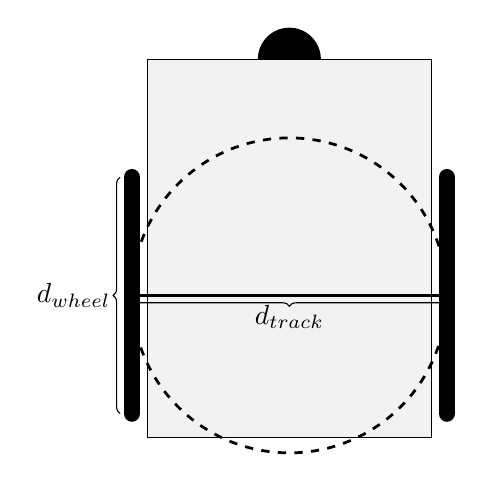
\begin{tikzpicture}
	\def\whDist{2}
	\def\whRad{1.5}
	\def\thirdWheel{3}
	\def\rectBound{0.3}
	
	% wheels
	\draw[line width=6pt, line cap=round] (-\whDist, -\whRad) -- (-\whDist, \whRad);
	\draw[line width=6pt, line cap=round] (\whDist, -\whRad) -- ( \whDist, \whRad);
	%third wheel circle
	\fill[line width = 1pt]  (0, \thirdWheel) circle (0.4);
	
	%robot box
	\draw[fill=gray!10] (-\whDist+0.2, -\whRad-\rectBound) rectangle (\whDist-0.2, \thirdWheel);
	
	% robot circle
	\draw[line width = 1pt, dashed]  (0, 0) circle (\whDist);
	
	%axis between wheels
	\draw[line width = 1pt]  (-\whDist, 0) -- (\whDist, 0);
	%distance decoration
	\draw[ decoration={brace}, decorate] (-\whDist-0.15, -\whRad) -- (-\whDist-0.15, \whRad) node[pos=0.5, anchor=east, ] {$d_{wheel}$};
	%wheel decoration
	\draw[ decoration={brace, mirror, raise=0.05cm}, decorate] (-\whDist, 0) -- (\whDist, 0) node[pos=0.5, anchor=north] {$d_{track}$};
	
	\end{tikzpicture}
	\caption{Robot wheel positioning}
	\label{fig:rb_wheel_graph}
\end{figure}
% optional new page
% to adjust figure
Assuming that our requirement is angle in degrees
$$
\theta_{dh} =  \frac{180}{\pi} \theta_{rh},   
$$
equation \ref{eq:rb_heading} can be simplified and robot heading in degrees can be calculated as
\begin{align*}
\theta_{dh} 
& = \frac{180}{\pi} (ce_{r} - ce_{l} ) \cdot rad_{pc} 								\\
& = \frac{180}{\pi} (ce_{r} - ce_{l} )   \frac{\pi}{180}\cdot \frac{ 50 }{ 224 } 	\\
& = (ce_{r} - ce_{l} ) \cdot \frac{ 50 }{ 224 } 									\\
& \Longrightarrow \\
\theta_{dh}
& = (ce_{r} - ce_{l} ) \cdot \frac{ d_{wheel} }{ 2\cdot d_{track} } .
\end{align*}

Having the left and right encoder counts, these equations enable to estimate wheeled robot's position.